\documentclass[11pt]{article}
\usepackage{../estilo-ejercicios}
\usepackage{wasysym}
\usetikzlibrary{automata,positioning}
\usepackage{mathdots}
\usepackage{listings}

\setlength{\parindent}{0em}
\setlength{\parskip}{1em}
\newcommand\tq{{\ \ /\ \ }}
\let \sii \Leftrightarrow
\let \luego \Rightarrow

\begin{document}
\begin{ejercicio}{1}
Definamos $F : \N^3\to \N$ por
$$F(x, e, t) = \text{valor de la variable }Y\text{ tras ejecutar el programa }e\text{ sobre }x\text{ durante }t\text{ pasos.}$$
Decimos que $x$ es un $F$-punto de $\varphi_e$ si $x \neq 0$ y para algún $t \in \N$, $F(x, e, t) = x$. Probar que:
\begin{enumerate}
\item $F$ es recursiva.
\item El conjunto $A = \{e \in \N : \varphi_e$ tiene un $F$-punto$\}$ es r.e.
\end{enumerate}
\end{ejercicio}
\begin{solucion}\
\begin{enumerate}
	\item $F(x,e,t)=(r(\texttt{di}(x,e,t))_1$, por lo que es primitiva recursiva.
	\item \[ A = \{ e \in \N : \exists x : F(x,e,t) = x \} \]
entonces:
\[ e \in A \sii \exists x \exists t : F(x,e,t) = x \]
Tomando $R(e,x) \sii F(x,e,t) = x$. Como $F$ es recursivo, $R$ es recursivo. Por el ejercicio 5.1 (consecuencia del teorema de proyección), $A$ es r.e.
\end{enumerate}
\end{solucion}

\newpage

\begin{ejercicio}{2}
Sea Prim $\subseteq \N$ el conjunto de los números primos. Pruébese que
\begin{enumerate}
\item El conjunto $A_1 = \{\#(P) : P$ es un programa $GOTO$ y rang$([\![P]\!]^{(1)})\subseteq$Prim$\}$ NO es un conjunto recursivo.
\item El conjunto $A_2 = \{e \in \N : \varphi_e(e)\in$Prim$\}$ es r.e. pero NO es recursivo.
\item El siguiente conjunto NO es r.e.
$$A_3 = \{e \in \N : (\forall x) [\varphi_e(x + e)\uparrow\lor \varphi_e(x)\uparrow \lor(\varphi_e(x + e)\downarrow \land \varphi_e(x)\downarrow \land \varphi_e(x + e) \neq \varphi_e(x))]\}$$
(Indicación: Utilícese el teorema del complemento y el teorema de recursión).
\end{enumerate}
\end{ejercicio}
\begin{solucion}\
\begin{enumerate}
	\item Sea
	\[  Γ = \{g \in \mathcal{P}^{(1)} : rang(g) \subseteq \text{Prim}\} \]
	Vemos que $Γ \neq \emptyset$ con el programa constante $2$ y vemos que $Γ \neq \mathcal{P}^{(1)}$ con el programa constante $1$. Entonces $A_1 = I_Γ$ es no recursivo por el teorema de Rice.
	
	\item Sea $\Gamma=\{ \varphi_e\in\mathcal{P}: \varphi_e(e)\in$Prim$\}$. Podemos usar las mismas funciones del apartado anterior, ya que al ser constantes sobre sus códigos dan los mismos resultados para probar por el teorema de Rice que $I_{\Gamma}=A_2$ no es recursivo.
	
	Respuesta alternativa para evitar el problema de que $\varphi$ pueda reconocer su código o no:
	Supongamos que es recursivo y sea la función 
	\[
	g(e,x)=\begin{cases}
	0 & e\in A_2\\
	2 & e\notin A_2
	\end{cases}
	\]
	Por la hipótesis que hemos supuesto $g(e,x)$ es recursiva, por lo que existe $\hat{e}$ tal que $g(\hat{e},x)=\varphi_{\hat{e}}(x)\ \forall x$. Si $\hat{e}\in A_2$ entonces $g(\hat{e},x)=\varphi_{\hat{e}}(x)=0\ \forall x$, en particular para $x=\hat{e}$, con lo que se llega a contradicción porque 0 no es primo. En caso contrario, $g(\hat{e},\hat{e})=\varphi_{\hat{e}}(\hat{e})=2$, que es primo, luego volvemos a tener contradicción.
	
	Para ver que es recursivamente enumerable vamos a ver que $\mathcal{K}$ es reducible a $A_2$. Sea $\mathcal{C}_3$ la función constantemente 3. Entonces $e\in\mathcal{K}\Leftrightarrow \mathcal{C}_3(e)\in A_2$. Como sabemos que $\mathcal{K}$ es r.e., entonces también lo es $A_2$. 
	
	\item Consideremos el complementario $\overline{A}_3$. Se va a probar que es r.e. y no recursivo, de modo que por el teorema del complemento, $A_3$ no puede ser r.e. Así pues, 
\begin{gather*}
e\in\overline{A}_2\sii (\exists x)[\varphi_e(x+e)\downarrow\land\varphi_e(x)\downarrow\land(\varphi_e(x+e)\uparrow\lor\varphi_e(x)\uparrow\lor \varphi_e(x+e)=\varphi_e(x))]\sii\\
\sii (\exists x)[\varphi_e(x+e)\downarrow\land\varphi_e(x)\downarrow\land\varphi_e(x+e)=\varphi_e(x))]
\end{gather*}
Sea ahora $g(u,v)=\mathcal{U}(v,u)$ recursiva, por el teorema de recursión existe $e$ tal que $\varphi_e(x)=g(e,x)=\mathcal{U}(x,e)$. En particular también $\varphi_e(x+e)=g(e,x+e)=\mathcal{U}(x+e,e)$. Sustituyendo esto en el predicado anterior deducimos que es recursivamente enumerable por ser un existencial sobre conjunciones de predicados r.e., y no recursivo (pues interviene el problema de la parada).
\end{enumerate}
\end{solucion}

\newpage
\begin{ejercicio}{3}
Se pide:
\begin{enumerate}
\item Dar una expresión regular que genere el lenguaje aceptado por el siguiente autómata finito:
\[ 
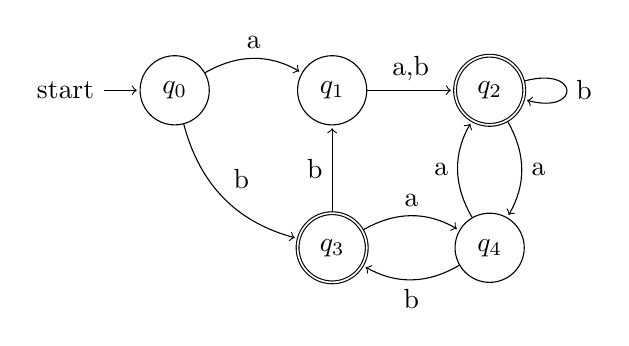
\begin{tikzpicture}[shorten >=1pt,node distance=2cm,on grid,auto] 
   \node[state,initial] (q_0)   {$q_0$}; 
   \node[state] (q_1) [right=of q_0] {$q_1$};
   \node[state,accepting] (q_2) [right=of q_1] {$q_2$};
   \node[state,accepting] (q_3) [below=of q_1] {$q_3$};
   \node[state] (q_4) [right=of q_3] {$q_4$};
    \path[->] 
    (q_0) edge [bend left] node {a} (q_1)
          edge [bend right] node {b} (q_3)
    (q_1) edge node {a,b} (q_2)
    (q_2) edge [bend left] node {a} (q_4)
          edge [loop right] node {b} ()
    (q_3) edge [bend left] node {a} (q_4)
          edge node {b} (q_1)
    (q_4) edge [bend left] node {b} (q_3)
          edge [bend left] node {a} (q_2);
\end{tikzpicture} \]

\item Construir un $\varepsilon$-AFND sobre el alfabeto $\{a, b, c\}$ que acepte el lenguaje generado por la
expresión regular $(ab^*c(ba)^* + (a + b)^*)^*$. ¿Acepta dicho autómata la palabra $bba$? ¿Y la
palabra $acb$? Razónense las respuestas.
\end{enumerate}
\end{ejercicio}
\begin{solucion}
\begin{enumerate}
\item 

\[ 
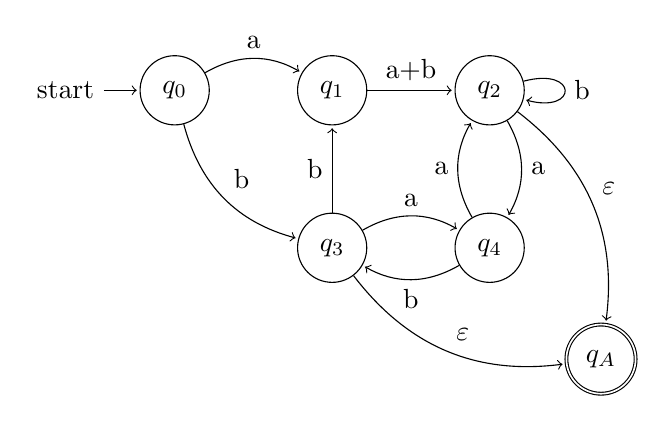
\begin{tikzpicture}[shorten >=1pt,node distance=2cm,on grid,auto] 
   \node[state,initial] (q_0)   {$q_0$}; 
   \node[state] (q_1) [right=of q_0] {$q_1$};
   \node[state] (q_2) [right=of q_1] {$q_2$};
   \node[state] (q_3) [below=of q_1] {$q_3$};
   \node[state] (q_4) [right=of q_3] {$q_4$};
   \node[state,accepting] (q_A) [below right=of q_4] {$q_A$};
    \path[->] 
    (q_0) edge [bend left] node {a} (q_1)
          edge [bend right] node {b} (q_3)
    (q_1) edge node {a+b} (q_2)
    (q_2) edge [bend left] node {a} (q_4)
          edge [loop right] node {b} ()
          edge [bend left] node {$\varepsilon$} (q_A)
    (q_3) edge [bend left] node {a} (q_4)
          edge node {b} (q_1)
          edge [bend right] node {$\varepsilon$} (q_A)
    (q_4) edge [bend left] node {b} (q_3)
          edge [bend left] node {a} (q_2);
\end{tikzpicture} \]
\[ 
\begin{tikzpicture}[shorten >=1pt,node distance=2cm,on grid,auto] 
   \node[state,initial] (q_0)   {$q_0$};
   \node[state] (q_2) [right=of q_1] {$q_2$};
   \node[state] (q_3) [below=of q_1] {$q_3$};
   \node[state] (q_4) [right=of q_3] {$q_4$};
   \node[state,accepting] (q_A) [below right=of q_4] {$q_A$};
    \path[->] 
    (q_0) edge [bend left] node {a(a+b)} (q_2)
          edge [bend right] node {b} (q_3)
    (q_2) edge [bend left] node {a} (q_4)
          edge [loop right] node {b} ()
          edge [bend left] node {$\varepsilon$} (q_A)
    (q_3) edge [bend left] node {a} (q_4)
          edge [bend left] node {b(a+b)} (q_2)
          edge [bend right] node {$\varepsilon$} (q_A)
    (q_4) edge [bend left] node {b} (q_3)
          edge [bend left] node {a} (q_2);
\end{tikzpicture} \]
\[ 
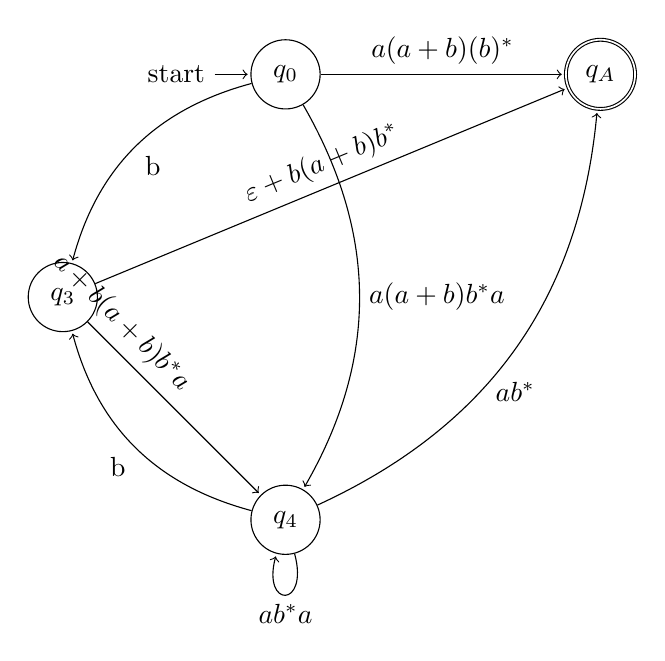
\begin{tikzpicture}[shorten >=1pt,node distance=4cm,on grid,auto] 
   \node[state,initial] (q_0)   {$q_0$};
   \node[state] (q_3) [below left=of q_0] {$q_3$};
   \node[state] (q_4) [below right=of q_3] {$q_4$};
   \node[state,accepting] (q_A) [right=of q_0] {$q_A$};
    \path[->] 
    (q_0) edge node {$a(a+b)(b)^*$} (q_A)
          edge [bend right] node {b} (q_3)
          edge [bend left] node {$a(a+b)b^*a$} (q_4)
    (q_3) edge node [pos=0.1,sloped] {$a+b(a+b)b^*a$} (q_4)
          edge node [sloped] {$\varepsilon+b(a+b)b^*$} (q_A)
    (q_4) edge [bend left] node {b} (q_3)
          edge [loop below] node {$ab^*a$} ()
          edge [bend right] node [below=0.3] {$ab^*$} (q_A);
\end{tikzpicture} \]

\[ 
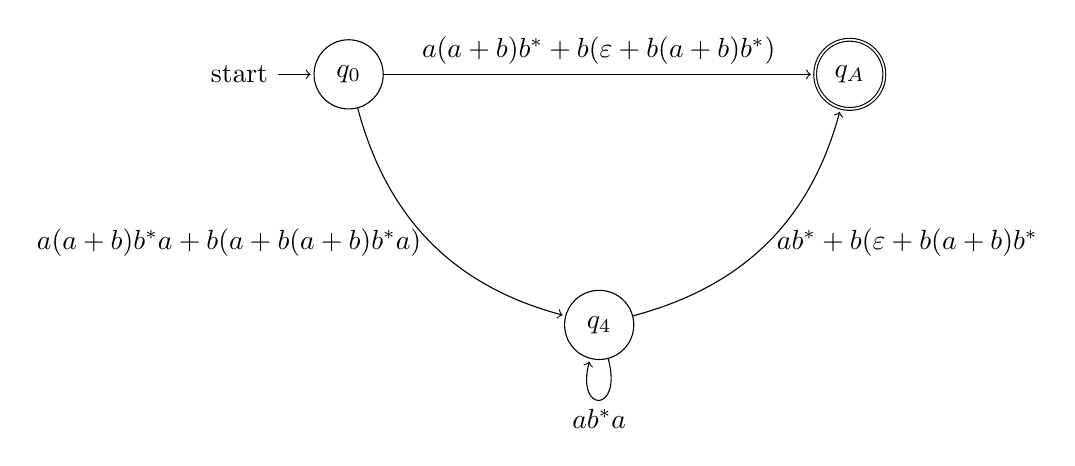
\begin{tikzpicture}[shorten >=1pt,node distance=4.5cm,on grid,auto] 
   \node[state,initial] (q_0)   {$q_0$};
   \node[state] (q_4) [below right=of q_0] {$q_4$};
   \node[state,accepting] (q_A) [above right=of q_4] {$q_A$};
    \path[->] 
    (q_0) edge node {$a(a+b)b^*+b(\varepsilon+b(a+b)b^*)$} (q_A)
          edge [bend right] node [left] {$a(a+b)b^*a+b(a+b(a+b)b^*a)$} (q_4)
    (q_4) edge [loop below] node {$ab^*a$} ()
          edge [bend right] node [right] {$ab^*+b(\varepsilon+b(a+b)b^*$} (q_A);
\end{tikzpicture} \]
Expresión regular:
\[ a(a+b)b^*+b(\varepsilon+b(a+b)b^*)+(a(a+b)b^*a+b(a+b(a+b)b^*a)(ab^*a)^*(ab^*+b(\varepsilon+b(a+b)b^*)\]
Quitando las $\varepsilon$:
\[ a(a+b)b^*+b+bb(a+b)b^*+(a(a+b)b^*a+b(a+b(a+b)b^*a)(ab^*a)^*(ab^*+b+bb(a+b)b^*)\]

\item 
\[ 
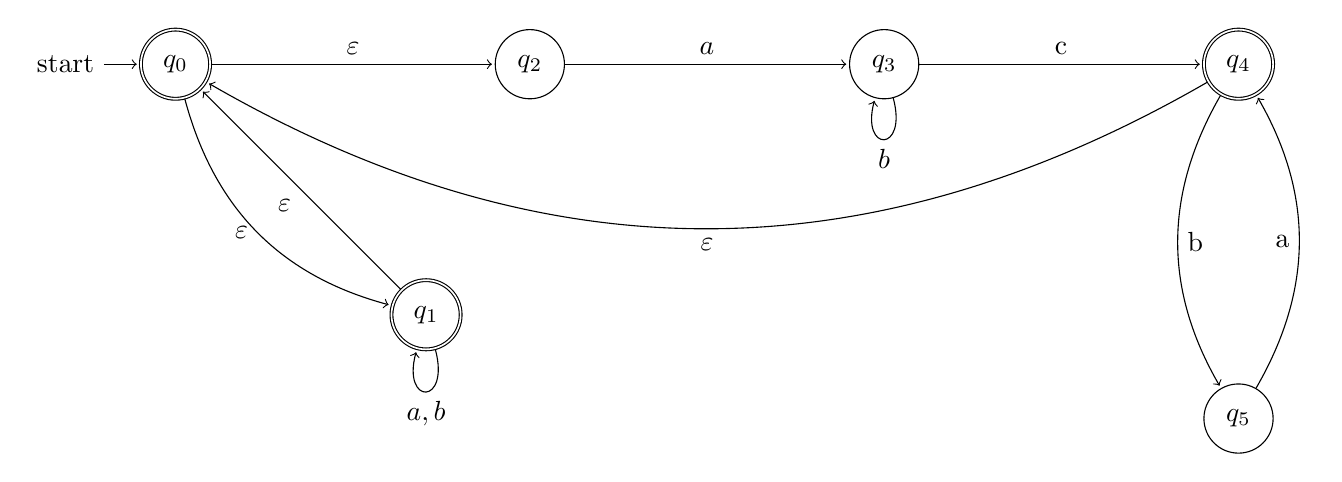
\begin{tikzpicture}[shorten >=1pt,node distance=4.5cm,on grid,auto] 
   \node[state,initial,accepting] (q_0)   {$q_0$};
   \node[state] (q_2) [right=of q_0] {$q_2$};
   \node[state, accepting] (q_1) [below right=of q_0] {$q_1$};
   \node[state] (q_3) [right=of q_2] {$q_3$};
   \node[state, accepting] (q_4) [right=of q_3] {$q_4$};
   \node[state] (q_5) [below=of q_4] {$q_5$};
    \path[->] 
    (q_0) edge node {$\varepsilon$} (q_2)
          edge [bend right] node  [left] {$\varepsilon$} (q_1)
    (q_1) edge [loop below] node {$a,b$} ()
          edge  node {$\varepsilon$} (q_0)
    (q_2)  edge  node {$a$} (q_3)
    (q_3) edge [loop below] node {$b$} ()
    	  edge node {c} (q_4)
    (q_4) edge [bend right] node {b} (q_5)
          edge [bend left] node {$\varepsilon$} (q_0)
     (q_5) edge [bend right] node {a} (q_4);
\end{tikzpicture} \]

Aceptará ambas palabras por forman parte del lenguaje aceptado anterior.
\end{enumerate}
\end{solucion}

\newpage

\begin{ejercicio}{4}
Consideremos el alfabeto $\Sigma=\{ a, b, c\}$. Se pide:
\begin{enumerate}
\item Probar, utilizando el lema del bombeo, que el siguiente lenguaje sobre $\Sigma$ no es regular:
$$L_1 = \{a^ib^jc^k : i, j, k \in \N, i + j = k\}$$
\item Probar que si $L\subseteq\Sigma^*$ es regular, el complementario de $L$, $\overline{L} = \{x \in \Sigma^* : x \notin L\}$ también
es regular.
\item Sea $L_2$ el lenguaje sobre $\Sigma$ generado por la expresión regular $a^*+b^*$. Construir un AFD que
acepte el complementario de $L_2$.

\end{enumerate}
\end{ejercicio}
\begin{solucion}\
\begin{enumerate}
\item Supongamos que $L_1$ es regular. Sea $n$ como en el lema del bombeo y sea $x=a^nb^jc^k$ con $j,k\in\N$ fijos Por hipótesis $n+j=k$. Entonces, por el lema del bombeo, $x=uvw$ con $|uv|\leq n$, $v\neq\varepsilon$ y $uv^rw\in L_1\ \forall r\in\N$. Como $v$ no es vacía y $|uv|\leq n$, se tiene que $v=a^m$ para cierto $m>0$. Entonces, tomando $r=0$ resulta que $uw\in L$, pero esto no es posible porque ha variado el número de $a$'s sin variar el resto de letras, por lo que no se cumple la igualdad $i+j=k$, donde $i$ sería el nuevo número de $a$'s. 

\item Sea $M=\langle Q,\Sigma, \delta, q_0,F\rangle$ un AFD que acepte el lenguaje $L$. Vamos a diseñar $\overline{M}=\langle Q,\Sigma,\delta,q_0, \overline{F}\rangle$ un AFD que acepte $\overline{L}$. Como hemos indicado, vamos a cambiar solo el conjunto de estados finales. Sea pues $\overline{F}=Q\setminus F$. Comprobemos su corrección. Sea $w\in\Sigma^*$, entonces $w\in L(\overline{M})\Leftrightarrow \hat{\delta}(q_0,w)\in\overline{F}\Leftrightarrow \hat{\delta}(q_0,w)\notin F\Leftrightarrow w\notin L(M)=L\Leftrightarrow w\in\overline{L}$.


\item Vamos a construirlo siguiendo el algoritmo descrito en el apartado anterior. Un AFD que aceptaría $a^*+b^*$ sería

\[ 
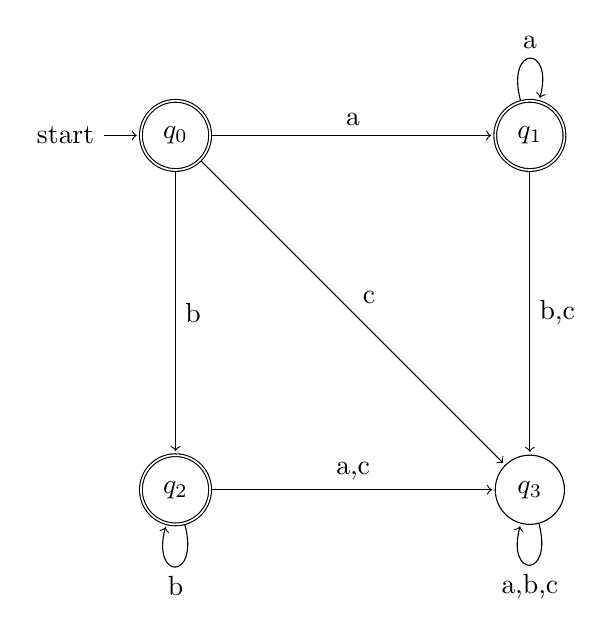
\begin{tikzpicture}[shorten >=1pt,node distance=4.5cm,on grid,auto] 
   \node[state,initial,accepting] (q_0)   {$q_0$};
   \node[state, accepting] (q_1) [right=of q_0] {$q_1$};
   \node[state, accepting] (q_2) [below =of q_0] {$q_2$};
   \node[state] (q_3) [below=of q_1] {$q_3$};
    \path[->] 
    (q_0) edge node {a} (q_1)
          edge node  {b} (q_2)
          edge node {c} (q_3)
    (q_1) edge [loop above] node {a} ()
          edge node {b,c} (q_3)
    (q_2) edge [loop below] node {b} ()
          edge node {a,c} (q_3)
    (q_3) edge [loop below] node {a,b,c} ();
\end{tikzpicture} \]

Por tanto, un AFD que acepte el complementario sería simplemente 

\[ 
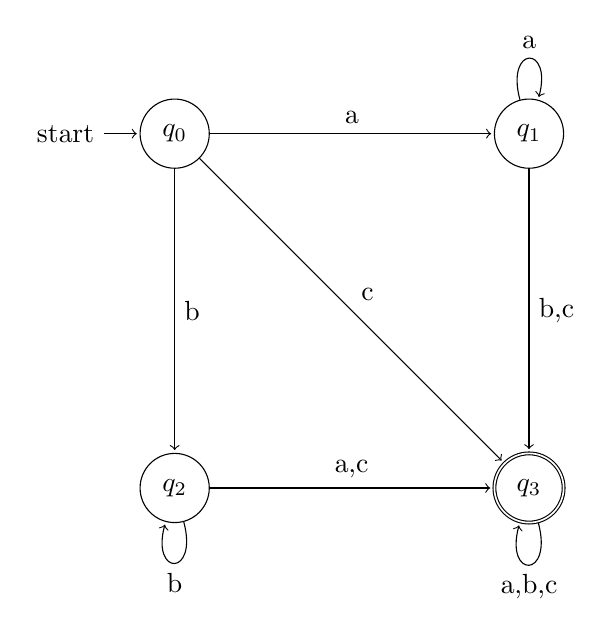
\begin{tikzpicture}[shorten >=1pt,node distance=4.5cm,on grid,auto] 
   \node[state,initial] (q_0)   {$q_0$};
   \node[state] (q_1) [right=of q_0] {$q_1$};
   \node[state] (q_2) [below =of q_0] {$q_2$};
   \node[state, accepting] (q_3) [below=of q_1] {$q_3$};
    \path[->] 
    (q_0) edge node {a} (q_1)
          edge node  {b} (q_2)
          edge node {c} (q_3)
    (q_1) edge [loop above] node {a} ()
          edge node {b,c} (q_3)
    (q_2) edge [loop below] node {b} ()
          edge node {a,c} (q_3)
    (q_3) edge [loop below] node {a,b,c} ();
\end{tikzpicture} \]
\end{enumerate}
\end{solucion}

\end{document}
